\documentclass[a4paper]{scrreprt}

%%% PACKAGES %%%

% add unicode support and use german as language
\usepackage[utf8]{inputenc}
\usepackage[ngerman]{babel}

% Use Helvetica as font
\usepackage[scaled]{helvet}
\renewcommand\familydefault{\sfdefault}
\usepackage[T1]{fontenc}

% Better tables
\usepackage{tabularx}

% Better enumerisation env
\usepackage{enumitem}

% Use graphics
\usepackage{graphicx}

% Have subfigures and captions
\usepackage{subcaption}

% Be able to include PDFs in the file
\usepackage{pdfpages}

% Have custom abstract heading
\usepackage{abstract}

% Need a list of equation
\usepackage{tocloft}
\usepackage{ragged2e}

% Better equation environment
\usepackage{amsmath}

% Symbols for most SI units
\usepackage{siunitx}

\usepackage{csquotes}

% Clickable Links to Websites and chapters
\usepackage{hyperref}

% Change page rotation
\usepackage{pdflscape}

% Symbols like checkmark
\usepackage{amssymb}
\usepackage{pifont}

% Bibliography & citing
\usepackage[
	backend=biber,
	style=apa,
	bibstyle=apa,
	citestyle=apa,
	sortlocale=de_DE
	]{biblatex}
\addbibresource{Referenzen.bib}
\DeclareLanguageMapping{ngerman}{ngerman-apa}

%%% COMMAND REBINDINGS %%%
\newcommand{\tabitem}{~~\llap{\textbullet}~~}
\newcommand{\xmark}{\ding{55}}

% Define list of equations - Thanks to Charles Clayton: https://tex.stackexchange.com/a/354096
\newcommand{\listequationsname}{\huge{Formelverzeichnis}}
\newlistof{myequations}{equ}{\listequationsname}
\newcommand{\myequations}[1]{
	\addcontentsline{equ}{myequations}{\protect\numberline{\theequation}#1}
}
\setlength{\cftmyequationsnumwidth}{2.3em}
\setlength{\cftmyequationsindent}{1.5em}

% Usage {equation}{caption}{label}
\newcommand{\indexequation}[3]{
	\begin{align} \label{#3} \ensuremath{\boxed{#1}} \end{align}
	\myequations{#3} \centering \small \textit{#2} \normalsize \justify }

%%% PATH DEFINITIONS %%%
% Define the path were images are found
\graphicspath{{./img/}{./pdf/}}

%%% DOCUMENT %%%

\begin{document}

\begin{titlepage}
	\begin{center}
		\vspace*{5cm}
		\Huge{\textbf{RFID markierte Exemplare}} \\
		\vspace{0.5em}
		\Large{Bachelordiplomarbeit FS2019}\\
		\vspace{3em}
		\LARGE{Pascal Baumann, Dane Wicki}\\
		\vspace{1em}
		\Large{Betreuer: Martin Jud}\\
		\vfill
		\large{Hochschule Luzern - Departement Informatik}\\
		\large{\today}\\
		\large{Version 0.1.0}
	\end{center}
\end{titlepage}

\pagenumbering{Roman}

\chapter*{Eidesstattliche Erklärung}
Ich erkläre hiermit, dass ich/wir die vorliegende Arbeit selbständig und ohne unerlaubte fremde Hilfe angefertigt haben, alle verwendeten Quellen, Literatur und andere Hilfsmittel angegeben haben, wörtlich oder inhaltlich entnommene Stellen als solche kenntlich gemacht haben, das Vertraulichkeitsinteresse des Auftraggebers wahren und die Urheberrechtsbestimmungen der Fachhochschule Zentralschweiz (siehe Merkblatt «Studentische Arbeiten» auf MyCampus) respektieren werden.

\vspace{1em}

\renewcommand{\arraystretch}{2}
\begin{tabularx}{\textwidth}{XXXX}
	Unterschrift: & 
\includegraphics[keepaspectratio, width=3cm]{PascalBaumann} & Unterschrift: & 
\includegraphics[keepaspectratio, width=3cm]{DaneWicki} \\ \cline{2-2}\cline{4-4}
	Baumann, Pascal & & Wicki, Dane & \\
	Datum: & \today & Ort: & Rotkreuz\\
\end{tabularx}
\renewcommand{\arraystretch}{1}

\renewcommand{\abstractname}{Management Summary}
\begin{abstract}
	Abstract
\end{abstract}

\tableofcontents

\clearpage
\pagenumbering{arabic}
\chapter{Einleitung}

\section{Aufgabenstellung und Zielsetzung}

\chapter{Stand der Technik}
\label{ch:StandDerTechnik}

\section{Technologische Grundlagen}

\section{Technische Konzepte}

\section{Anwendungen}

\chapter{Ideen und Konzepte}

\section{Grundidee}

\section{Lösungskonzept 1}

\section{Lösungskonzept 2}

\chapter{Methode}

\section{Projektinformationen}

\subsection{Vorgehensmodell}

Alle Wirtschaftsprojekte an der Hochschule Luzern fallen in eine der folgenden Kategorien:

\begin{enumerate}
	\item Einsatz von Standardsoftware und Services
	\item Software- und Produktentwicklung
	\item Innovationsprojekt
	\item IT-Infrastrukturentwicklung
	\item Strukturierte Analyse und Konzeption von Systemen und Abläufen
\end{enumerate}

Dabei ist dieses Projekt als Innovationsprojekt und Softwareentwicklung klassifiziert worden. Wir erwarteten daher unter anderem, eine Evaluation, Recherchen und weitere Unbekannten. Um auf diese eingehen zu können, entschied sich das Team dafür die hybride, inkrementelle Agile Methode zu verwenden.

\subsection{Agile Projektmethode}

Die agile Projektmethode zielt darauf ab in einem ungewissen und sich verändernden Umfeld zu bestehen. Insbesondere bedeutet dies, das auf sich verändernde Voraussetzungen schnell reagiert werden kann und dabei ein funktionierendes Produkt entsteht \parencite{AgileAlliance2015}. Dies soll durch eine enge Zusammenarbeit mit dem Auftraggeber und guter teaminterner Kommunikation erreicht werden.

\parencite{BaumannWicki2018}

\subsection{Ermittlung offener Projektrahmenbedingungen}
\label{ch:evaluation}

\subsection{Projektanforderungen}
Mittels einer Machbarkeitsstudie und einem Proof of Concept soll untersucht werden ob es möglich ist bis zu 120 RFID Tags in einem Behälter mit der Dimension 600x400x320mm zu identifizieren.

\begin{itemize}
	\item Es sollen mindestens zwei Lösungskonzepte für eine als Auswahl der Machbarkeitsstudie entwickelt werden.
	\item Die Lösungskonzepte müssen auf deren technische Realisierbarkeit untersucht werden.
	\item Es muss mindestens ein entwickeltes Konzept für die Machbarkeitsstudie verwendet werden.
	\item Die Machbarkeitsstudie muss eine Kostenrechnung für die Lösungsansätze beinhalten.
	\item Es soll eine MVP entwickelt werden, welches vom Kunde verwendet werden kann.
\end{itemize}

\subsubsection{Anforderungen an Lösungsansätze, Proof of Concept und MVP}

\begin{itemize}
	\item Die Lösungskonzepte müssen mit dem Lagersystem kommunizieren können
	\item Die Lösungskonzepte müssen die RFID Tags in weniger als 1 Sekunden identifizieren können.
	\item Die Lösungskonzepte müssen für das bestehende Hochregallager der Speicherbibliothek verwendbar sein.
	
	\item Das Proof of Concept muss technisch aufzeigen, wie viele RFID Tags in einer Sekunde gelesen werden können.
	\item Das Proof of Concept soll eine RFID Lesezuverlässigkeit von 95\% aufweisen.
	
	\item Das MVP soll mit der Datenbank des Lagersystems kommunizieren können.
	\item Das MVP soll in einem von Störfaktoren bereinigten Zustand die gleiche Anzahl RFID Tags lesen können wie im Proof of Concept definiert.
	\item Das MVP soll erkennen, wenn eine Box ein Exemplar enthält, welches nicht dieser Box zugehörig ist und dies als eine Unstimmigkeit markieren.
	\item Das MVP soll in der Lage sein, dem Endbenutzer in beliebiger Form mitzuteilen, welcher Behälter eine Unstimmigkeit enthält.
\end{itemize}

\subsection{Einschränkungen und Abgrenzungen}

\newpage
\section{Systemspezifikation}
\label{sec:SysSpec}

\subsection{Anforderungen}
\label{ch:Anforderungen}

\subsection{Kontext}

\subsection{Komponentendesign}

\subsection{Architektur \& Design}

\subsection{Interne Schnittstellen}

\subsection{Klassendiagramm}

\subsection{Anforderungen der Software}

\subsection{Umsetzung Programmierung}

\section{Testing}

\subsection{Testfälle}

\section{Machbarkeitsstudie}

\chapter{Realisierung}

\section{Applikationsablauf}

\chapter{Projektmanagementplan}

\section{Projektorganisation}

\vspace{1em}

\begin{tabularx}{\textwidth}{|X|X|}
	\hline
	\textbf{Projektbeteiligte} & \textbf{Funktionen} \\
	\hline
	Mike Märki & Stakeholder/Auftraggeber \\
	\hline
	Martin Jud & BDA Experte \\
	\hline
	Pascal Baumann & Product Owner \& Dev Team \\
	\hline
	Dane Wicki & Scrum Master \& Dev Team \\
	\hline
\end{tabularx}

\subsection{Organigramm}
\begin{figure}[h!]
	\centering
	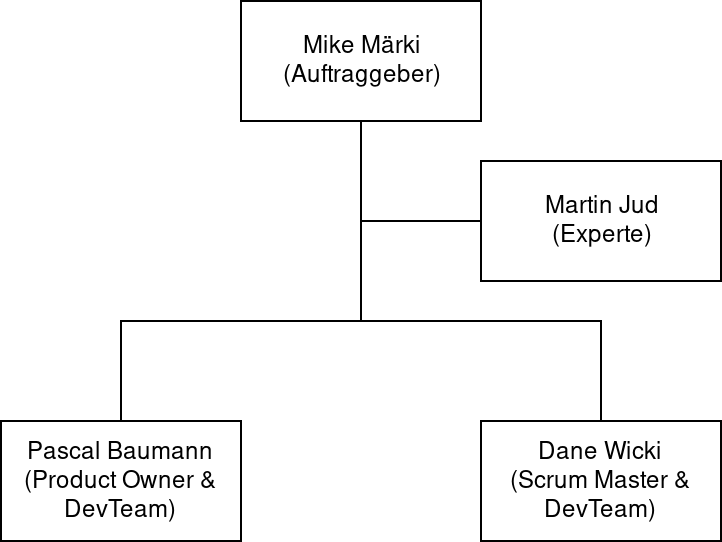
\includegraphics[keepaspectratio, width=0.6\textwidth]{OrganigrammBDA_BAWI.png}
\end{figure}


\section{Rahmenplan}
\subsection{Meilensteine}
\label{ssec:Meilensteine}
Für das Projekt wurden vier Meilensteine definiert, welche jeweils im Vierwochenzyklus auftreten. Diese Meilensteine sind in Abbildung \ref{fig:Milestones} dargestellt.

\begin{figure}[h!]
	\centering
	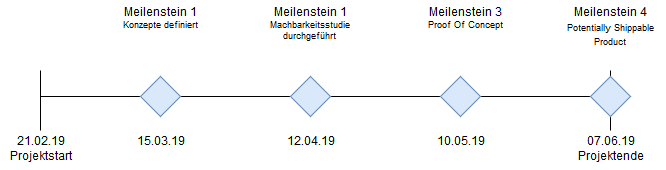
\includegraphics[keepaspectratio,width=0.8\linewidth]{Milestones.png}
	\caption{Die für das Projekt definierten Meilensteine}
	\label{fig:Milestones}
\end{figure}

\subsection{Grobplan}

Aus den im Kapitel \ref{ssec:Meilensteine} definierten Meilensteine wurden acht Sprints von zwei Wochen abgeleitet. In diesen werden sowohl die Artefakte wie Projektdokumentation, Machbarkeitsstudien und Systemspezifikation, wie auch das Produkt entwickelt. Der grobe Rahmenplan ist in Abbildung \ref{fig:Rahmenplan_1} dargestellt.

\begin{figure}[h!]
	\centering
	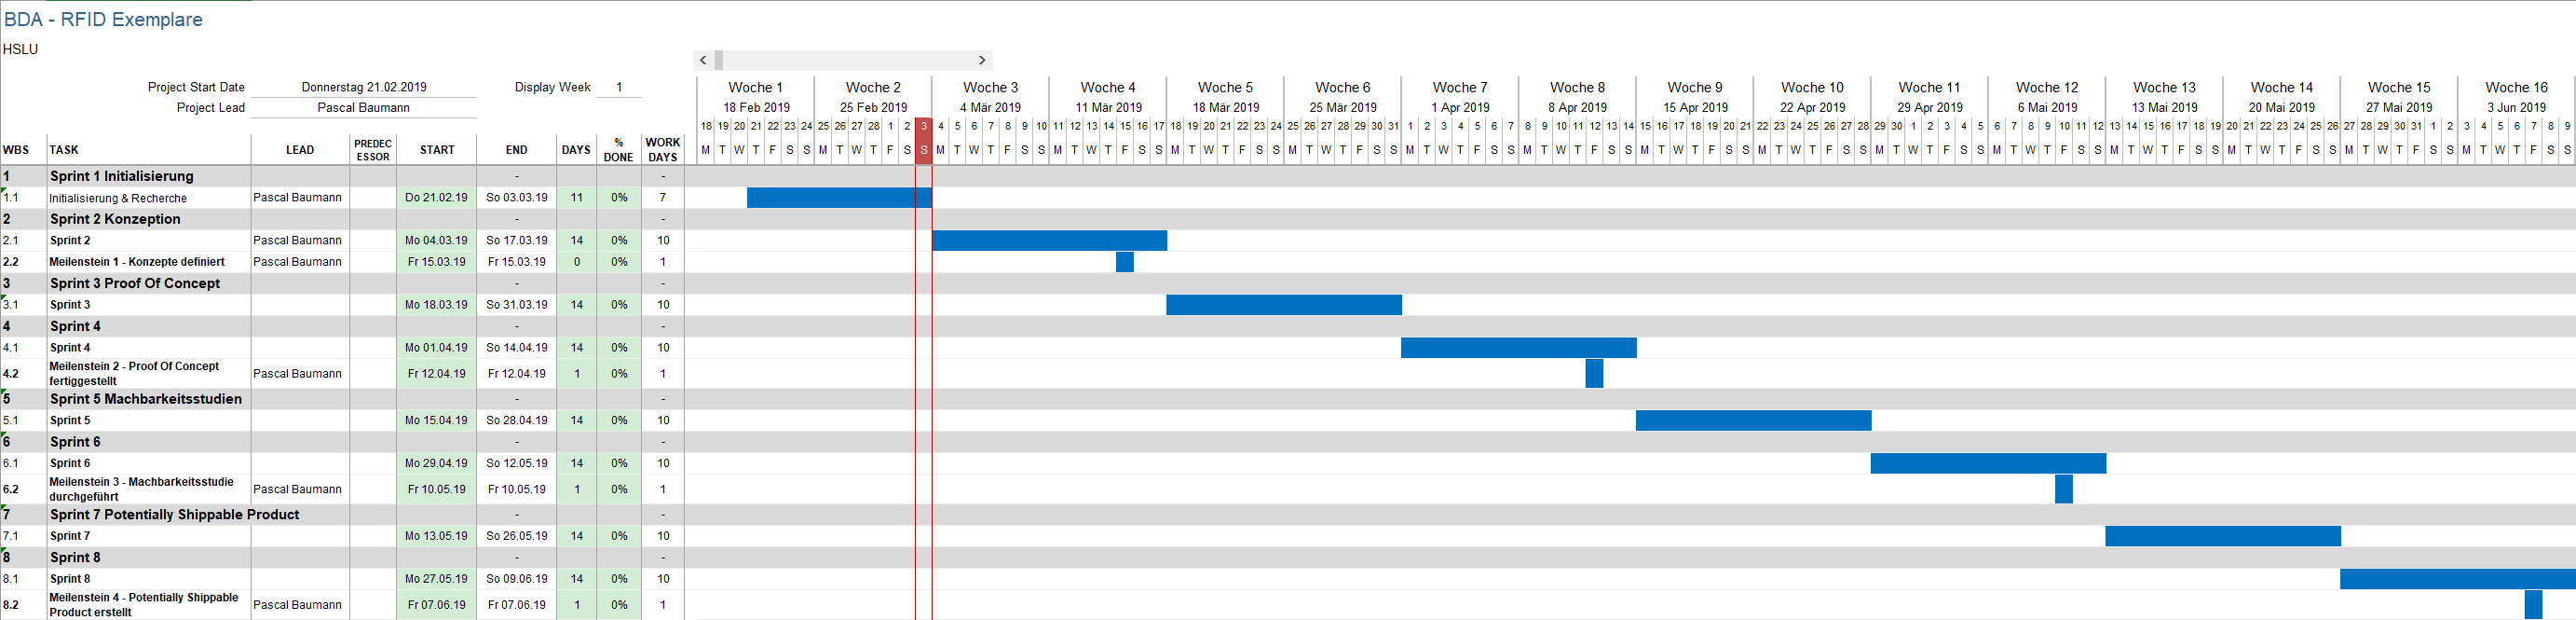
\includegraphics[keepaspectratio,width=\linewidth]{Grobplan.png}
	\caption{Übersicht der Sprints im Rahmenplan}
	\label{fig:Rahmenplan_1}
\end{figure}

\newpage

\section{Risikomanagement}

Es werden mögliche Risiken, welche während dem Projekt auftreten können aufgezählt. Diese werden auf Eintrittswahrscheinlichkeit und Schadensmass eingeschätzt, danach wird entschieden, welche Massnahmen getroffen werden können, und was deren Auswirkungen sind.

\subsection{Definitionen}
\label{sssec:Def}
\vspace{1em}
\noindent
Eintrittswahrscheinlichkeit:

\vspace{1em}
\noindent
\begin{tabularx}{\textwidth}{|l|l|X|}
	\hline
	\textbf{Stufe} & \textbf{Bezeichnung} & \textbf{Beschreibung} \\
	\hline
	1 & unvorstellbar & Möglich aber eher unwahrscheinlich. Tritt nie oder einmal in 16 Wochen auf \\
	\hline
	2 & unwahrscheinlich & Kann in 16 Wochen kein oder ein Mal eintreten\\
	\hline
	3 & vorstellbar & Kann in 16 Wochen ein bis zwei Mal eintreten \\
	\hline
	4 & wahrscheinlich & Kann in 16 Wochen bis zu drei Mal eintreten \\
	\hline
	5 & häufig & Kann in 16 Wochen sieben Mal eintreten\\
	\hline
\end{tabularx}

\vspace{1em}
\noindent
Schadensausmass:

\vspace{1em}
\noindent
\begin{tabularx}{\textwidth}{|l|l|X|}
	\hline
	\textbf{Stufe} & \textbf{Bezeichnung} & \textbf{Beschreibung} \\
	\hline
	1 & unwesentlich & Die Aufgabenerfüllung wird höchstens geringfügig beeinträchtigt, finanzieller Schaden ist im Rahmen des Projekts nicht beeinflussend. Personenschäden treten nicht auf. \\
	\hline
	2 & geringfügig & Wahrnehmbare Gefährdung / Einfluss auf das Projekt. Personenschäden treten nicht auf. \\
	\hline
	3 & mittelmässig & Wahrnehmbare Gefährdung / Einfluss auf das Projekt. Verzögerungen zur Folge. Finanzieller Schaden strapaziert das Projektbudget. Personenschäden treten nicht auf. \\
	\hline
	4 & kritisch & Starke Gefährdung des Projekts. Extreme Verzögerungen zur Folge. Finanzieller Schaden übersteigt das Projektbudget. Personenschäden treten geringfügig auf.\\
	\hline
	5 & katastrophal & Projektabbruch zur Folge. Finanzieller Schaden kann zum Projektstopp führen. Verletzung der Persönlichkeitsrechte. \\
	\hline
\end{tabularx}

\newpage

\subsection{Risikokatalog}
\label{sssec:Risikokatalog}
Legende:
\begin{itemize}
	\item \textbf{S}chadensausmass bei Eintreffen des Risikos
	\item \textbf{W}ahrscheinlichkeit das Risiko eintrifft
	\item \textbf{K}ategorie: \textbf{T}echnisches oder \textbf{P}rojektbezogenes Risiko
	\item \textbf{A}uswirkung auf das Projekt. Produkt aus S und W
\end{itemize}

\vspace{1em}
\noindent
\begin{table}[htb]
	\begin{tabularx}{\textwidth}{|l|X|l|l|l||l|}
		\hline
		\textbf{Nr.} & \textbf{Beschreibung / Risiko} & \textbf{K} & \textbf{S} & \textbf{W} & \textbf{A} \\
		\hline
		1 & Meilensteine werden nicht erreicht & P & 4 & 2 & 8 \\
		\hline
		2 & Teammitglied fällt aus & P & 4 & 1 & 4 \\
		\hline
		3 & Fehlkommunikation im Team & P & 4 & 1 & 4 \\
		\hline
		4 & Produkt entspricht nicht den Kundenanforderungen & P & 5 & 2 & 10 \\
		\hline
		5 & Umsetzung des Produkts technisch nicht möglich & T & 4 & 3 & 12 \\
		\hline
		6 & Datenverlust & T & 5 & 2 & 10 \\
		\hline
		7 & Lieferschwierigkeiten von Teilen & P & 3 & 3 & 9 \\
		\hline
	\end{tabularx}
	\caption{Die im Projekt identifizierten Risiken}
	\label{tbl:Risks}
\end{table}

\vspace{1em}

\begin{figure}[h!]
	\centering
	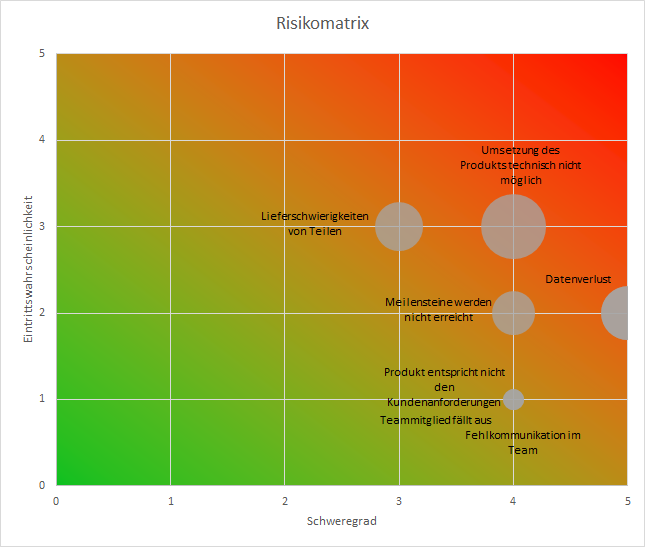
\includegraphics[keepaspectratio, width=0.6\textwidth]{Risks_before.png}
	\caption{Auswirkungen der in Tabelle \ref{tbl:Risks} identifizierten Risiken}
\end{figure}

\newpage

\subsubsection{Massnahmen}

\begin{table}[htb]
	\begin{tabularx}{\textwidth}{|l|X|}
		\hline
		\textbf{Nr.} & \textbf{Beschreibung Massnahme} \\
		\hline
		1 & Meilensteine werden in zwei Zweiwöchigen Sprints absolviert. Die Tasks pro Sprint werden weiter detailliert heruntergebrochen. So sollen die Arbeiten sowohl auf Makro- wie Mikrosicht eingeplant werden. \\
		\hline
		2 & Arbeiten werden so strukturiert und dokumentiert, dass das zweite Mitglied diese auch übernehmen kann. Es werden Spezialisierungen der Teammitglieder insoweit verhindert, dass Wissenslücken minimiert werden. Recherchen sollen Zusammenfassungen und Merkblätter über die gewonnenen Erkenntnisse als Resultat haben.\\
		\hline
		3 & Der Kontakt wird von beiden Teammitgliedern sowohl horizontal im Team wie auch vertikal zu den Stakeholdern aktiv gesucht. Es werden den Arbeiten auch teambildende Aktivitäten zusammen absolviert.\\
		\hline
		4 & Der Kunde muss den Fortschritt alle vier Wochen in einer Sitzung kontrollieren, avisieren und, wenn nötig, Anpassungen fordern.\\
		\hline
		5 & Es soll während den Recherchen schon im Hinblick auf die technische Umsetzung acht gegeben werden.\\
		\hline
		6 & Sowohl produzierten Artefakte, wie auch aktuelle getätigte Arbeiten werden auf auswärtige Plattformen ausgelagert.\\
		\hline
		7 & Teile werden bei Bedarf sofort bestellt, es werden inländische, etablierte Lieferanten, vor evtl. günstigeren Ausländischen vorgezogen.\\
		\hline
	\end{tabularx}
	\caption{Massnahmen um Effekte oder Eintrittswahrscheinlichkeit zu reduzieren}
\end{table}

\vspace{1em}

\begin{table}[htb]
	\begin{tabularx}{\textwidth}{|l|X|l|l|l||l|}
		\hline
		\textbf{Nr.} & \textbf{Beschreibung / Risiko} & \textbf{K} & \textbf{S} & \textbf{W} & \textbf{A} \\
		\hline
		1 & Meilensteine werden nicht erreicht & P & 4 & 1 & 4 \\
		\hline
		2 & Teammitglied fällt aus & P & 3 & 1 & 3 \\
		\hline
		3 & Fehlkommunikation im Team & P & 4 & 1 & 4 \\
		\hline
		4 & Produkt entspricht nicht den Kundenanforderungen & P & 5 & 1 & 5 \\
		\hline
		5 & Umsetzung des Produkts technisch nicht möglich & T & 4 & 3 & 12 \\
		\hline
		6 & Datenverlust & T & 5 & 1 & 5 \\
		\hline
		7 & Lieferschwierigkeiten von Teilen & P & 3 & 2 & 6 \\
		\hline
	\end{tabularx}
	\caption{Neueinschätzung der Risiken nach Einführung der Massnahmen}
	\label{tbl:Massnahmen}
\end{table}

\vspace{1em}

\begin{figure}[h!]
	\centering
	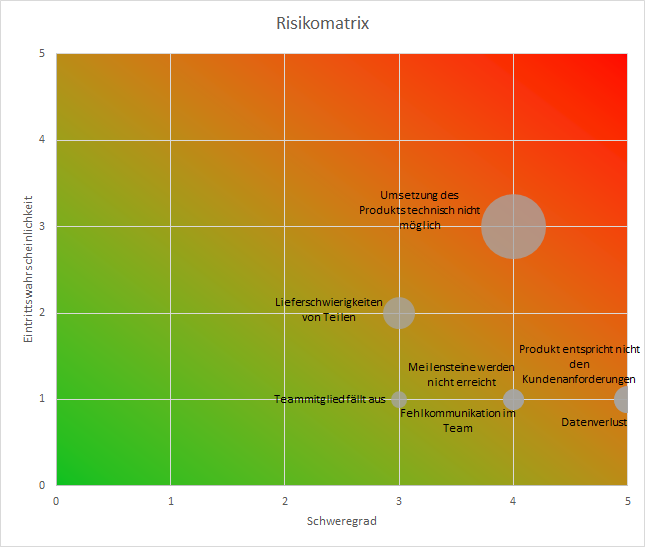
\includegraphics[keepaspectratio, width=0.6\textwidth]{Risks_after.png}
	\caption{Auswirkungen der Risiken nach den in Tabelle \ref{tbl:Massnahmen} vorgeschlagenen Massnahmen}
\end{figure}

\chapter{Evaluation und Validation}
\label{ch:Eval}

\section{Vergleich mit Anforderungen}
\label{sec:VergleichAnforderungen}

\chapter{Ausblick}
\label{ch:Ausblick}

\section{Projekt Fazit}

\newpage

\pagenumbering{Roman}

\appendix

\glossary{Abkürzungsverzeichnis}

\listoffigures

\listoftables

\listofmyequations \pagebreak

\printbibliography

\end{document}
